\begin{ZhChapter}
    \chapter{Related Work}
    In the following section, we will introduce the concept of metaheuristics \cite{yang2010nature,yang2011metaheuristic} and explain how they are used to solve real-life problems. Then, we will discuss the importance of loss functions and their role in deep learning \cite{deepLearning} models. Finally, we will explore image classification and its real-life applications.

    \section{Metaheuristic}
    Metaheuristic was first proposed by ... this concept means we can ...


    Evolving algorithm \cite{muhlenbein1988evolution}, genetic algorithm and genetic programming \cite{geneticProgramming} are algorithms using the concept of Metaheuristic, we will introduce them in the following paragraph.

    Evolving algorithm was first proposed in ...

    The concept of genetic algorithm was proposed and .....

    Genetic programming, can be seen as one of the special case of genetic algorithm, has been used in different domain because it doesn't require specific domain knowledge to implement.

    In \cite{coreyes2022evolvingreinforcementlearningalgorithms}, \citeauthor{coreyes2022evolvingreinforcementlearningalgorithms} proposed a meta-learning reinforcement learning algorithm. They used computational graphs to represent algorithms. By doing so, algorithms could be identified, calculated, and optimized through Reinforcement Learning (RL) \cite{kaelbling1996reinforcement}. Notably, in this study, algorithms were represented as directed acyclic graphs (DAG) \cite{thost2021directedacyclicgraphneural} of nodes. Within the DAG , all nodes were classified into three categories: input nodes, parameter nodes, and operation nodes. Once the algorithms were represented as DAGs, they could be placed into RL for training and evaluation. In this proposed algorithm, they employed the concept of regularized evolution \cite{real2019regularized} to evolve a population formed by several randomized and known algorithms. The method was as follows: initialize the population with algorithms, evaluate each algorithm in the population and record their performance, then in a loop, repeatedly use a sample tournament \cite{goldberg1991comparative} to select algorithms, perform mutations on the algorithms by the mutator they designed, and evaluate them again until the loop ends. During the evaluation process, they trained and assessed the algorithms using RL, continuously testing the performance of each algorithm in different training environments. They also utilized normalized training performance to avoid numerical biases caused by varying environments. Through this approach, the study successfully created two algorithms, named DQNClipped and DQNReg, which outperformed classical control tasks.

    In \cite{akhmedova2024generationlossfunctionimage}, \citeauthor{akhmedova2024generationlossfunctionimage} proposed a genetic programming-based method to find a better function for the image classification training task. They encoded the loss functions into trees, with each tree considered an individual. All individuals were aggregated into a population. In this study, the population was evolved across multiple generations. Before the start of each generation, all individuals were evaluated. Each individual had a probability of undergoing crossover with an individual from a special external archive to create a new individual; otherwise, it would perform the crossover with another individual. Following this, two probabilistic decisions were made. If successful, the new individual could perform subtree mutation or one-point mutation, respectively. At the end of each generation, the fitness value of all individuals was re-evaluated. A certain number of low-scoring individuals were eliminated to the special external archive mentioned earlier, maintaining the stability of the population's size. After these steps, a new generation began, continuing until a predefined number of generations was reached.  By employing this method, this study successfully evolved an outstanding individual within the population, creating a function that could train an image classification model more effectively compared to Cross Entropy (CE) \cite{zhang2018generalized}.

    \section{Loss Function}

    \subsection{Deep Learning Model}

    \subsection{Importance of Loss Function}
    In \cite{gonzalez2020improvedtrainingspeedaccuracy}, a loss function meet genetic programming is proposed ....
    \section{Image Classification}

    % \subsection{}
    % 定義定義定義定義定義定義\cite{latex2e},定義定義定義定義,定義定義定義定義定義定義定義定義定義定義,定義定義。

    % \begin{table*}[htbp]
    %     \centering
    %     \caption{表格範例標題} \label{tab: complexity}
    %     \makebox[\linewidth][c]{
    %     \renewcommand\arraystretch{1.2}{
    %         \begin{tabular}{| l | c  c  c  c |}
    %         \hline
    %         Protocol & $P$ & $CS_1$ & $CS_2$ & $RG$ \\
    %         \hline
    %         MSSMul & $O(1)$, $O(1)$, N/A & $O(n-t)$, $O(n)$, $O(1)$ & $O(n-t)$, $O(n)$, N/A & $O(1)$, $O(n)$, $O(n)$ \\
    %         SC & $O(1)$, $O(1)$, N/A & $O(n-t)$, $O(n)$, $O(1)$ & $O(n-t)$, $O(n)$, N/A & $O(1)$, $O(n)$, $O(n)$ \\
    %         \hline 
    %         \end {tabular}
    %     }}
    % \end {table*}

    % \section{模型說明(小標)}

    % 說明說明說明說明,說明說明說明說明說明說明說明說明說明說明說明說明,說明說明說明說明說明說明說明說明。

    % \begin{figure*}[htbp]
    %     \centering
    %     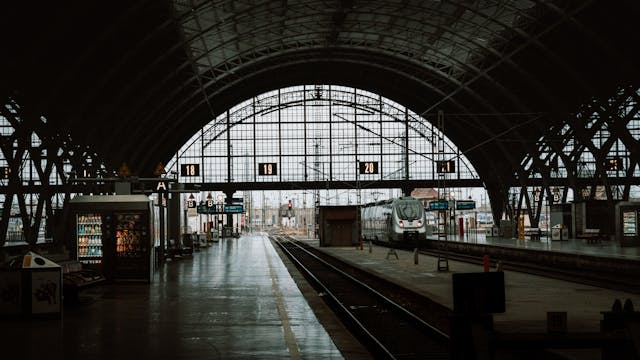
\includegraphics[width = 0.5\textwidth]{image.jpeg}
    %     \caption{Cool train station}
    %     \label{fig: image}
    % \end{figure*}

\end{ZhChapter}